\chapter{Selection Efficiencies, 2018}
\label{chap:eff_2018}

Here we study the efficiencies and purities in the same way as \autoref{sec:ND280:sel}, using unweighted raw Monte-Carlo events.

\section{$\nu_\mu$ in FHC}
Since the FHC selection is unchanged to the 2017 analysis, the efficiency and purities are very similar and here we only compare FGD1 CC0$\pi$ in 2018 to 2017 in \autoref{fig:fgd1_cc0pi_eff_2017_2018}, and refer to \autoref{tab:eff_pur_summary_2018} for the summary.
\begin{figure}[h]
	\centering
	\caption*{2018 analysis}
	\begin{subfigure}[t]{\textwidth}
		\centering
		\begin{subfigure}[t]{0.4\textwidth}
			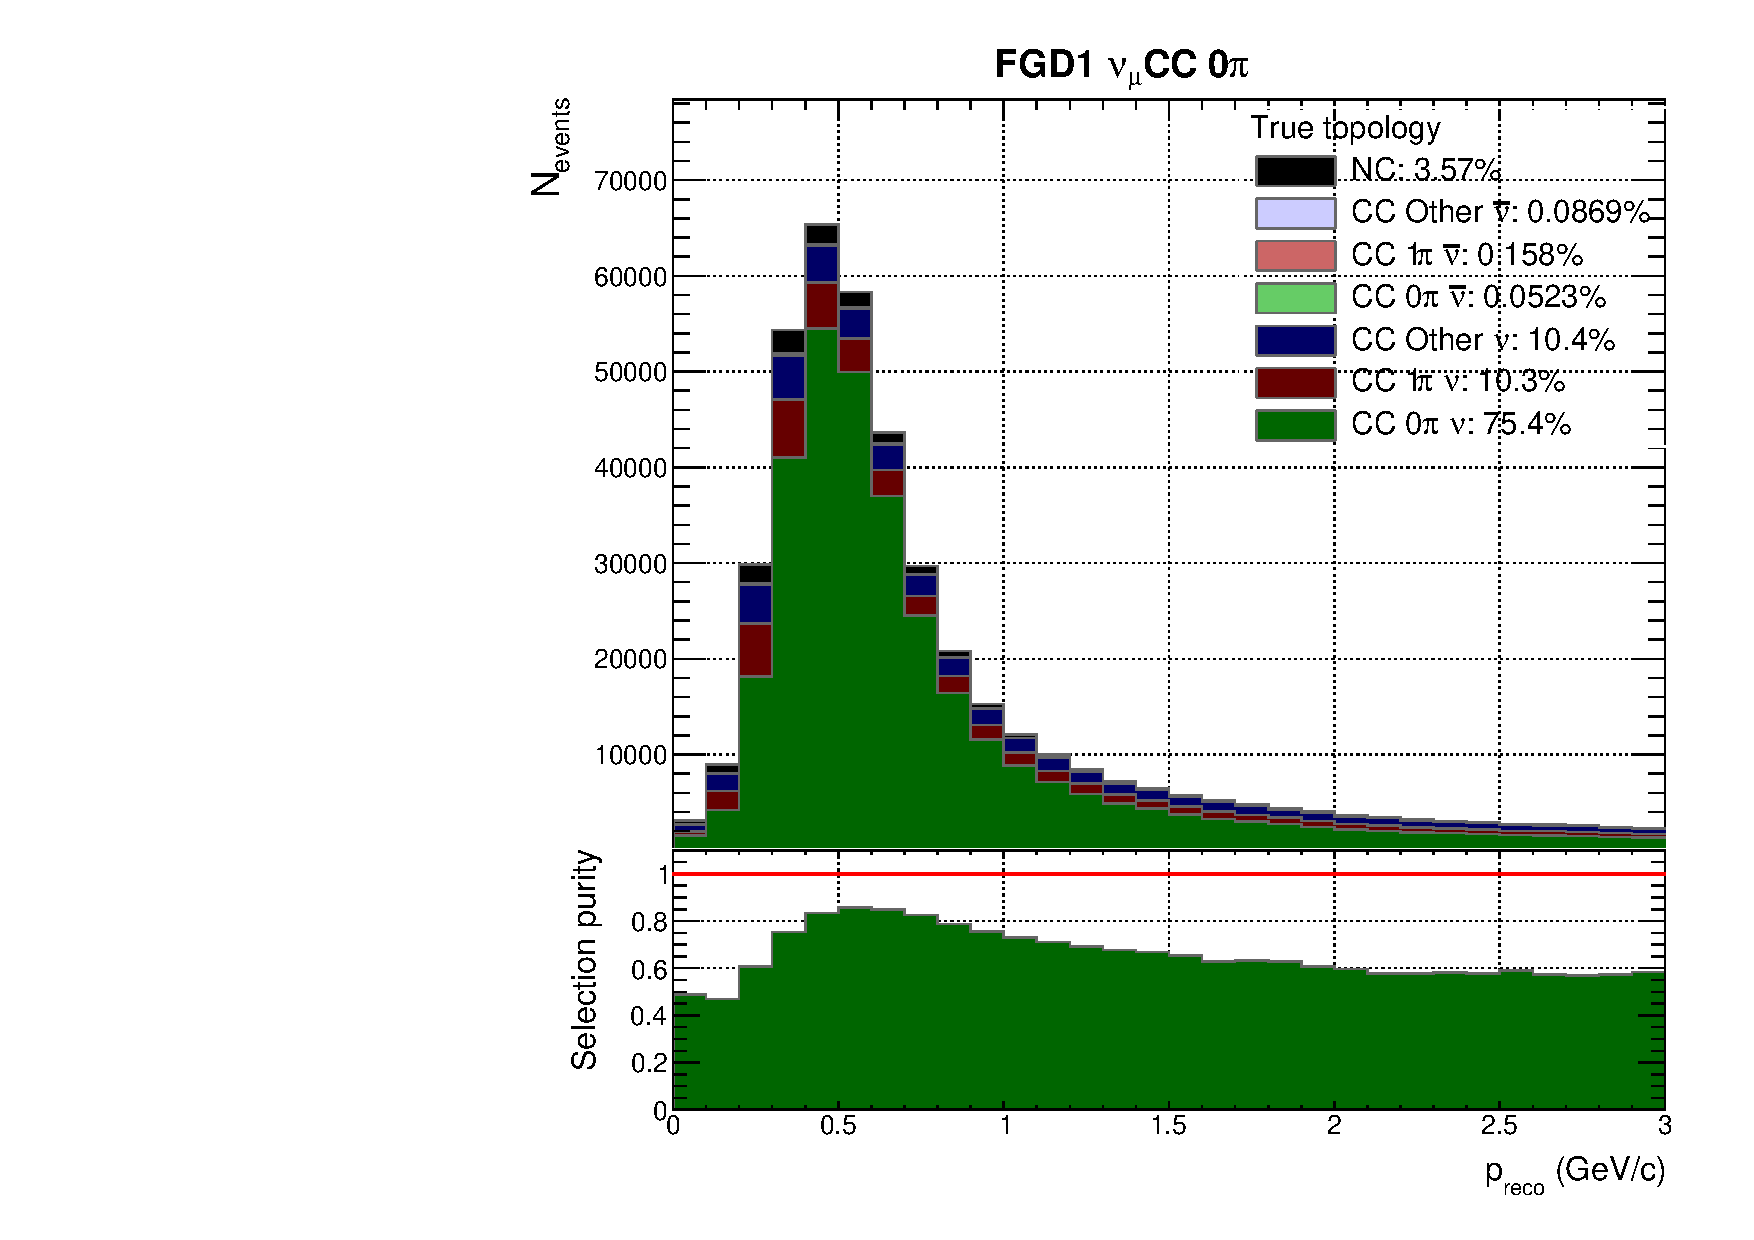
\includegraphics[width=\textwidth,page=1, trim={0mm 0mm 0mm 9mm}, clip]{figures/mach3/2018/Selection/2018_RedNDmatrix_rebin_verbose_may_noweights_diagnostics}
			\caption{Efficiency}
		\end{subfigure}
		\begin{subfigure}[t]{0.4\textwidth}
			\includegraphics[width=\textwidth,page=2, trim={0mm 0mm 0mm 9mm}, clip]{figures/mach3/2018/Selection/2018_RedNDmatrix_rebin_verbose_may_noweights_diagnostics}
			\caption{Purity}
		\end{subfigure}
	\end{subfigure}
	
	\begin{subfigure}[t]{\textwidth}
		\centering
		\caption*{2017 analysis}
		\begin{subfigure}[t]{0.4\textwidth}
			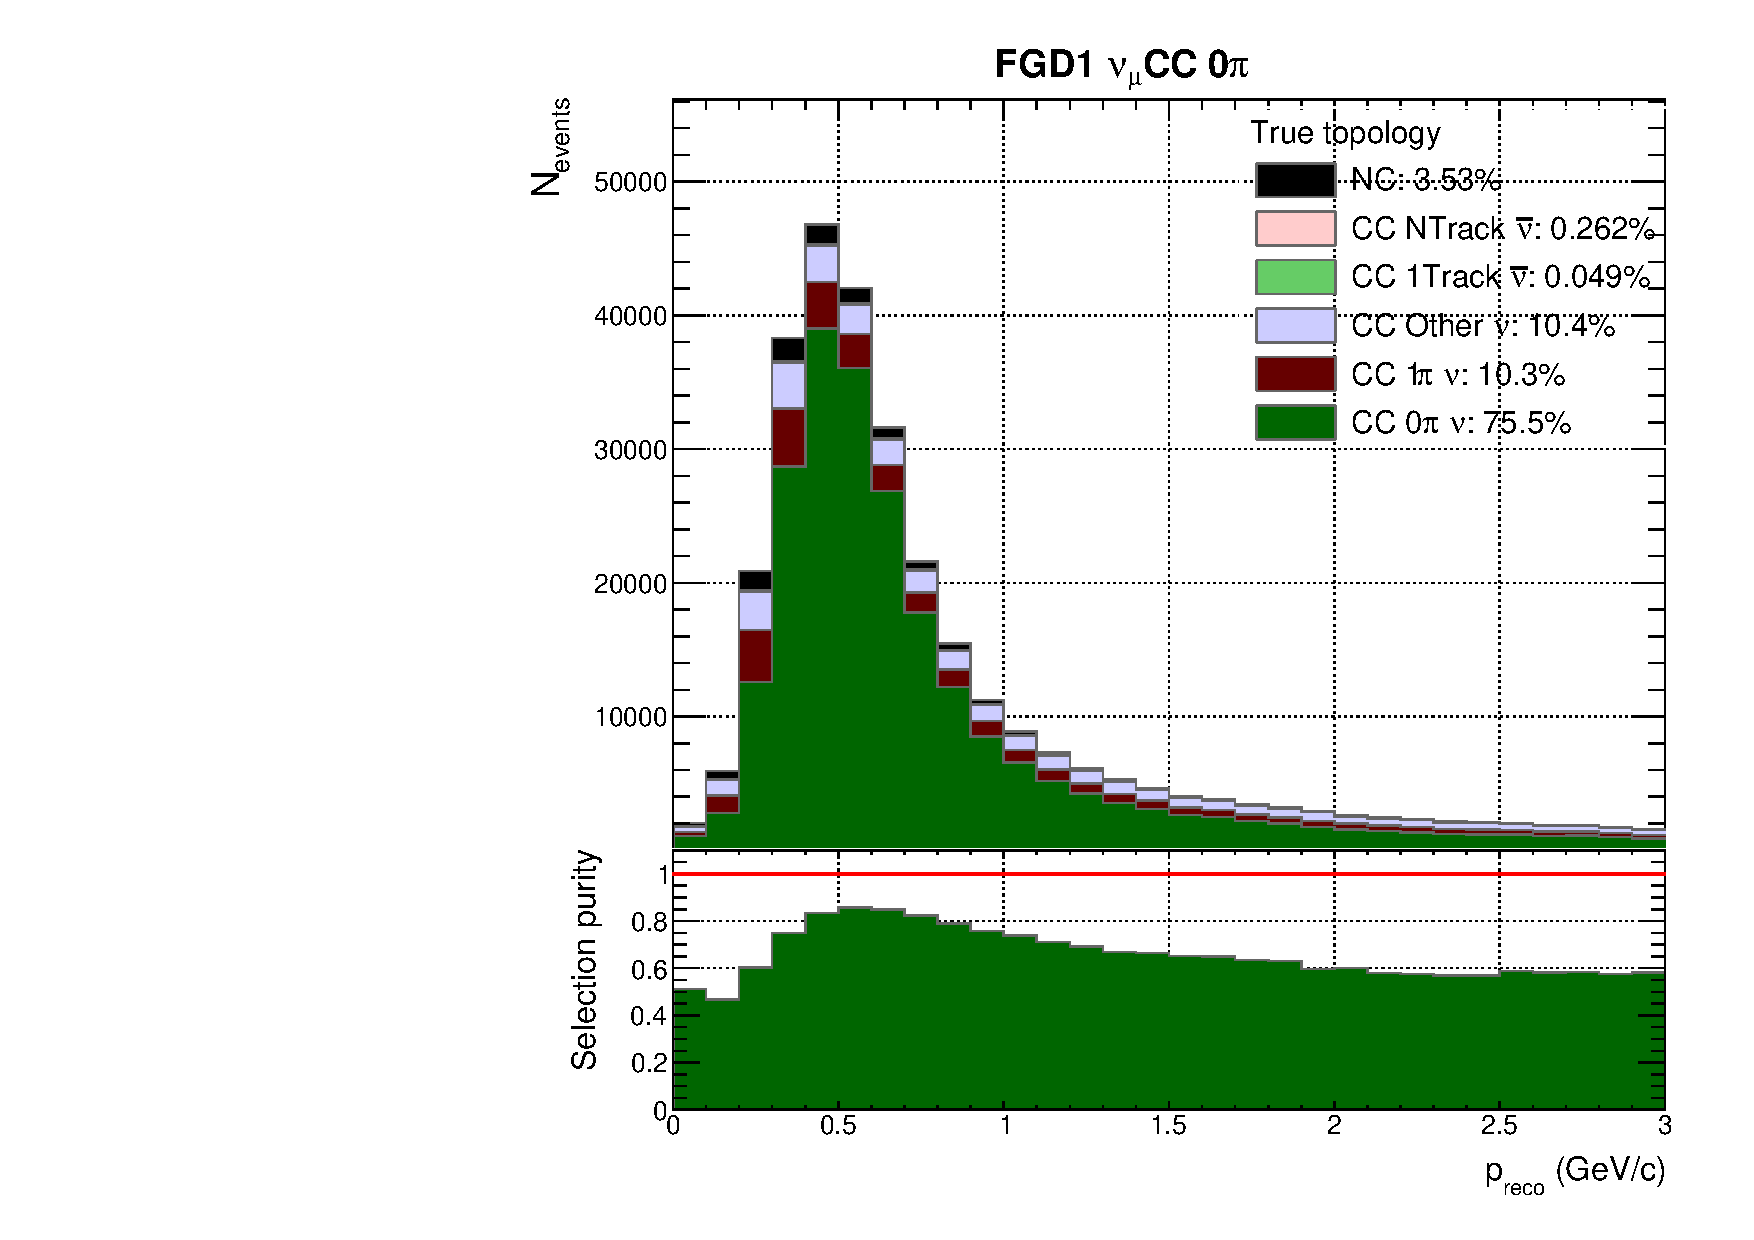
\includegraphics[width=\textwidth,page=1, trim={0mm 0mm 0mm 9mm}, clip]{figures/mach3/selection/2017b_Diag_WithSelection}
			\caption{Efficiency}
		\end{subfigure}
		\begin{subfigure}[t]{0.4\textwidth}
			\includegraphics[width=\textwidth,page=2, trim={0mm 0mm 0mm 9mm}, clip]{figures/mach3/selection/2017b_Diag_WithSelection}
			\caption{Purity}
		\end{subfigure}
	\end{subfigure}
	\caption{FGD1 0$\pi$ efficiencies and purities for 2017 and 2018 analyses}
	\label{fig:fgd1_cc0pi_eff_2017_2018}
\end{figure}

\section{$\bar{\nu}_\mu$ in RHC}
The CC0$\pi$ RHC selections are much the same as the 2017 1Track selection, and as such the purity in \autoref{fig:numubar_cc0pi_topology_2018} is almost identical to \autoref{fig:ccnubar1trk_topology}. Both FGDs have similar purities and the largest contamination is right-sign single events in which the pion is missed, at about 9.5\%. The NC contribution is 5\% and the total wrong-sign contribution is $\sim5\%$, similar to the 1Trk selection. The difference comes primarily from the removed upper bound on the muon likelihood cut. Moving up in momentum, the purity reduces to about 60\% from 85\% at the event peak.
\begin{figure}[h]
	\begin{subfigure}[t]{0.49\textwidth}
		\includegraphics[width=\textwidth,page=13, trim={0mm 0mm 0mm 9mm}, clip]{figures/mach3/2018/Selection/2018_RedNDmatrix_rebin_verbose_may_noweights_diagnostics}
		\caption{FGD1}
	\end{subfigure}
	\begin{subfigure}[t]{0.49\textwidth}
		\includegraphics[width=\textwidth,page=19, trim={0mm 0mm 0mm 9mm}, clip]{figures/mach3/2018/Selection/2018_RedNDmatrix_rebin_verbose_may_noweights_diagnostics}
		\caption{FGD2}
	\end{subfigure}
	\caption{Breakdown of \numubar CC0$\pi$ selection events' true event topology for FGD1 and FGD2 }
	\label{fig:numubar_cc0pi_topology_2018}
\end{figure}

\autoref{fig:numubar_cc0pi_muon_2018} shows the muon tagging efficiency, which again is comparable to the 1Trk equivalent in \autoref{fig:ccnubar1trk_muon}. The largest mis-id comes from $\pi^+$ being reconstructed as the muon, and the wrong-sign contamination is small. At $\sim1.5\text{ GeV}$ we see the characteristic proton bump---which makes up 3\% of the total---in which the dE/dx of a proton is very similar to that of a muon, causing it to be the selected highest momentum positive track with a muon likelihood.
\begin{figure}[h]
	\begin{subfigure}[t]{0.49\textwidth}
		\includegraphics[width=\textwidth,page=14, trim={0mm 0mm 0mm 9mm}, clip]{figures/mach3/2018/Selection/2018_RedNDmatrix_rebin_verbose_may_noweights_diagnostics}
		\caption{FGD1}
	\end{subfigure}
	\begin{subfigure}[t]{0.49\textwidth}
		\includegraphics[width=\textwidth,page=20, trim={0mm 0mm 0mm 9mm}, clip]{figures/mach3/2018/Selection/2018_RedNDmatrix_rebin_verbose_may_noweights_diagnostics}
		\caption{FGD2}
	\end{subfigure}
	\caption{Breakdown of \numubar CC0$\pi$ selection events' true lepton candidate for FGD1 and FGD2}
	\label{fig:numubar_cc0pi_muon_2018}
\end{figure}

Moving to the 1$\pi$ \numubar selection, the purity is shown in \autoref{fig:numubar_cc1pi_topology_2018}. The \numubar RHC selection sees similar performance to the \numu FHC equivalent in \autoref{fig:cc1pi_topology}, reaching an overall purity of $50-54\%$, with FGD1 being the higher. The wrong-sign contamination is significant at 25-30\%, coming from a $\pi^+$ in a CC1$\pi^+$ or CC DIS event being reconstructed as the muon candidate, and the $\mu^-$ reconstructed as the $\pi^-$. The right-sign CCOther contamination is about 10\%, owing mostly to one or several missed $\pi$. We again see the CC0$\pi$ \numu peak at 1.5 GeV, where the proton (likely from a CCQE or 2p2h interaction) is reconstructed as the $\mu^+$.
\begin{figure}[h]
	\begin{subfigure}[t]{0.49\textwidth}
		\includegraphics[width=\textwidth,page=15, trim={0mm 0mm 0mm 9mm}, clip]{figures/mach3/2018/Selection/2018_RedNDmatrix_rebin_verbose_may_noweights_diagnostics}
		\caption{FGD1}
	\end{subfigure}
	\begin{subfigure}[t]{0.49\textwidth}
		\includegraphics[width=\textwidth,page=21, trim={0mm 0mm 0mm 9mm}, clip]{figures/mach3/2018/Selection/2018_RedNDmatrix_rebin_verbose_may_noweights_diagnostics}
		\caption{FGD2}
	\end{subfigure}
	\caption{Breakdown of \numubar CC1$\pi$ selection events' true event topology for FGD1 and FGD2 }
	\label{fig:numubar_cc1pi_topology_2018}
\end{figure}

\autoref{fig:numubar_cc1pi_muon_2018} shows the muon tagging efficiency, which in the event peak sits at 80\% and decreases to 50\% with increasing $p_{\text{reco}}$. Tagging the right-sign pion as the lepton candidate happens 20\% of the time, and protons at $p\sim1.5\text{ GeV}$ about 15\% of the time, making up a large fraction of mis-identification. However, the 1$\pi$ selection is still almost 10\% more efficient and pure than the old CCNTrack selection.
\begin{figure}[h]
	\begin{subfigure}[t]{0.49\textwidth}
		\includegraphics[width=\textwidth,page=16, trim={0mm 0mm 0mm 9mm}, clip]{figures/mach3/2018/Selection/2018_RedNDmatrix_rebin_verbose_may_noweights_diagnostics}
		\caption{FGD1}
	\end{subfigure}
	\begin{subfigure}[t]{0.49\textwidth}
		\includegraphics[width=\textwidth,page=22, trim={0mm 0mm 0mm 9mm}, clip]{figures/mach3/2018/Selection/2018_RedNDmatrix_rebin_verbose_may_noweights_diagnostics}
		\caption{FGD2}
	\end{subfigure}
	\caption{Breakdown of \numubar CC1$\pi$ selection events' true lepton candidate for FGD1 and FGD2}
	\label{fig:numubar_cc1pi_muon_2018}
\end{figure}

Finally \autoref{fig:numubar_ccOth_topology_2018} shows the purity of the \numubar CCOther selection, which collects all \numubar CC candidates that weren't classified as CC0$\pi$ or CC1$\pi$. As with the equivalent \numu selection, the sample suffers from low purity due to broken tracks and secondary interactions, leading to a mis-reconstructed number of pions in the event. The selection has an almost equal efficiency for \numubar CCOther events as it does for \numu CCOther events, and in FGD2 it's indeed more pure of wrong-sign events. It has a high NC contamination due to collecting high pion multiplicity events, causing a pion to be reconstructed as a muon in the TPC.  At low momentum, the purity is close to zero, being swamped by wrong-sign 0$\pi$ events in which the low momentum $\mu^-$ is identified as a $\mu^+$, owing to the changed likelihood cut which in the 2017 analysis was present to remove such events. The wrong-sign 0$\pi$ and 1$\pi$ contributions largely vanish above 500 MeV and the wrong sign component is almost exclusively \numu CCOther.
\begin{figure}[h]
	\begin{subfigure}[t]{0.49\textwidth}
		\includegraphics[width=\textwidth,page=17, trim={0mm 0mm 0mm 9mm}, clip]{figures/mach3/2018/Selection/2018_RedNDmatrix_rebin_verbose_may_noweights_diagnostics}
		\caption{FGD1}
	\end{subfigure}
	\begin{subfigure}[t]{0.49\textwidth}
		\includegraphics[width=\textwidth,page=23, trim={0mm 0mm 0mm 9mm}, clip]{figures/mach3/2018/Selection/2018_RedNDmatrix_rebin_verbose_may_noweights_diagnostics}
		\caption{FGD2}
	\end{subfigure}
	\caption{Breakdown of \numubar CCOther selection events' true event topology for FGD1 and FGD2 }
	\label{fig:numubar_ccOth_topology_2018}
\end{figure}

The muon tagging efficiency of the \numubar CCOther selection is shown in \autoref{fig:numubar_ccOth_muon_2018}, which echoes the conclusions above. The efficiency is below 50\% and has almost equal parts proton tagging and $\pi^+$ tagging as contaminants. The wrong sign tag happens primarily at low momentum, in which the charge is reconstructed in the magnetic field. The proton bump at 1.5 GeV is especially present in this selection.
\begin{figure}[h]
	\begin{subfigure}[t]{0.49\textwidth}
		\includegraphics[width=\textwidth,page=18, trim={0mm 0mm 0mm 9mm}, clip]{figures/mach3/2018/Selection/2018_RedNDmatrix_rebin_verbose_may_noweights_diagnostics}
		\caption{FGD1}
	\end{subfigure}
	\begin{subfigure}[t]{0.49\textwidth}
		\includegraphics[width=\textwidth,page=24, trim={0mm 0mm 0mm 9mm}, clip]{figures/mach3/2018/Selection/2018_RedNDmatrix_rebin_verbose_may_noweights_diagnostics}
		\caption{FGD2}
	\end{subfigure}
	\caption{Breakdown of \numubar CCOther selection events' true lepton candidate for FGD1 and FGD2}
	\label{fig:numubar_ccOth_muon_2018}
\end{figure}

\section{$\nu_\mu$ in RHC}
As with the \numubar CC0$\pi$ selection, the \numu RHC CC0$\pi$ selection is largely identical to the 1Track equivalent in the 2017 analysis. The purity in \autoref{fig:numurhc_cc0pi_topology_2018} is above 53\%, with large contamination from right-sign 1$\pi$ and Other interactions, and the wrong-sign background making up 8\%, slightly less than the 1Track case. The NC contamination is almost identical to the 1Track selection at 9\%. We note the purity above 600 MeV stabilises at about 60\%.
\begin{figure}[h]
	\begin{subfigure}[t]{0.49\textwidth}
		\includegraphics[width=\textwidth,page=25, trim={0mm 0mm 0mm 9mm}, clip]{figures/mach3/2018/Selection/2018_RedNDmatrix_rebin_verbose_may_noweights_diagnostics}
		\caption{FGD1}
	\end{subfigure}
	\begin{subfigure}[t]{0.49\textwidth}
		\includegraphics[width=\textwidth,page=31, trim={0mm 0mm 0mm 9mm}, clip]{figures/mach3/2018/Selection/2018_RedNDmatrix_rebin_verbose_may_noweights_diagnostics}
		\caption{FGD2}
	\end{subfigure}
	\caption{Breakdown of \numu RHC CC0$\pi$ selection events' true event topology for FGD1 and FGD2 }
	\label{fig:numurhc_cc0pi_topology_2018}
\end{figure}

The muon tagging efficiency is shown in \autoref{fig:numurhc_cc0pi_muon_2018}, where we note 90\% above 1 GeV. At the event peak the efficiency sits at 55\%, leading to overall 78\%. In and below the event peak the main contamination is from $\pi^-$ (13\%) and as we go down in momentum the wrong-sign contributions increase due to wrongly reconstructing the charge in the magnet. At low momentum the wrong-sign component is $\times10$ larger than the right-sign.
\begin{figure}[h]
	\begin{subfigure}[t]{0.49\textwidth}
		\includegraphics[width=\textwidth,page=26, trim={0mm 0mm 0mm 9mm}, clip]{figures/mach3/2018/Selection/2018_RedNDmatrix_rebin_verbose_may_noweights_diagnostics}
		\caption{FGD1}
	\end{subfigure}
	\begin{subfigure}[t]{0.49\textwidth}
		\includegraphics[width=\textwidth,page=32, trim={0mm 0mm 0mm 9mm}, clip]{figures/mach3/2018/Selection/2018_RedNDmatrix_rebin_verbose_may_noweights_diagnostics}
		\caption{FGD2}
	\end{subfigure}
	\caption{Breakdown of \numu RHC CC0$\pi$ selection events' true lepton candidate for FGD1 and FGD2}
	\label{fig:numurhc_cc0pi_muon_2018}
\end{figure}

The CC1$\pi$ purity is shown in \autoref{fig:numurhc_cc1pi_topology_2018}, where we again see a large wrong-sign contribution at low momentum, primarily from \numubar 1$\pi$ events. The purity is 43\% overall, and a meagre 20\% in the event peak. The right-sign CCOther amount is constant with momentum, making up almost 1/3 at higher momentum.
\begin{figure}[h]
	\begin{subfigure}[t]{0.49\textwidth}
		\includegraphics[width=\textwidth,page=27, trim={0mm 0mm 0mm 9mm}, clip]{figures/mach3/2018/Selection/2018_RedNDmatrix_rebin_verbose_may_noweights_diagnostics}
		\caption{FGD1}
	\end{subfigure}
	\begin{subfigure}[t]{0.49\textwidth}
		\includegraphics[width=\textwidth,page=33, trim={0mm 0mm 0mm 9mm}, clip]{figures/mach3/2018/Selection/2018_RedNDmatrix_rebin_verbose_may_noweights_diagnostics}
		\caption{FGD2}
	\end{subfigure}
	\caption{Breakdown of \numu RHC CC1$\pi$ selection events' true event topology for FGD1 and FGD2 }
	\label{fig:numurhc_cc1pi_topology_2018}
\end{figure}

The muon tagging efficiency in \autoref{fig:numurhc_cc1pi_muon_2018} performs similarly to the NTrack selection at 65\%. At the event peak the efficiency is barely 20\%--the rest split almost equally amongst $\pi^-$, $\pi^+$ and $\mu^+$---but increases steadily to 85\% at higher momentum, where to wrong-sign component vanishes. The total wrong-sign contribution is 12\% but is dominant at low momentum. The $\pi^-$ contribution is sizeable at 22\%, which dies off at higher momentum.
\begin{figure}[h]
	\begin{subfigure}[t]{0.49\textwidth}
		\includegraphics[width=\textwidth,page=28, trim={0mm 0mm 0mm 9mm}, clip]{figures/mach3/2018/Selection/2018_RedNDmatrix_rebin_verbose_may_noweights_diagnostics}
		\caption{FGD1}
	\end{subfigure}
	\begin{subfigure}[t]{0.49\textwidth}
		\includegraphics[width=\textwidth,page=34, trim={0mm 0mm 0mm 9mm}, clip]{figures/mach3/2018/Selection/2018_RedNDmatrix_rebin_verbose_may_noweights_diagnostics}
		\caption{FGD2}
	\end{subfigure}
	\caption{Breakdown of \numu RHC CC1$\pi$ selection events' true lepton candidate for FGD1 and FGD2}
	\label{fig:numurhc_cc1pi_muon_2018}
\end{figure}

The \numu RHC CCOther selection's purity seen in \autoref{fig:numurhc_ccOth_topology_2018} is relatively high compared to other CC Other selection; overall 61\%. At low momentum the NC contribution is the largest, which is also the largest background overall at 13\%. Interestingly, the right-sign 0$\pi$ selection contaminates the sample 10\% and is the second largest contamination. Since the sign selection looks for a negative track for \numu selections, the CC0$\pi$ contribution can not come from a proton track being the muon candidate, and must be broken tracks being reconstructed as multiple pions.
\begin{figure}[h]
	\begin{subfigure}[t]{0.49\textwidth}
		\includegraphics[width=\textwidth,page=29, trim={0mm 0mm 0mm 9mm}, clip]{figures/mach3/2018/Selection/2018_RedNDmatrix_rebin_verbose_may_noweights_diagnostics}
		\caption{FGD1}
	\end{subfigure}
	\begin{subfigure}[t]{0.49\textwidth}
		\includegraphics[width=\textwidth,page=35, trim={0mm 0mm 0mm 9mm}, clip]{figures/mach3/2018/Selection/2018_RedNDmatrix_rebin_verbose_may_noweights_diagnostics}
		\caption{FGD2}
	\end{subfigure}
	\caption{Breakdown of \numu RHC CCOther selection events' true event topology for FGD1 and FGD2 }
	\label{fig:numurhc_ccOth_topology_2018}
\end{figure}

The corresponding muon efficiency is shown in \autoref{fig:numurhc_ccOth_muon_2018}, where we see close to zero efficiency at low momentum. In this region the electron is the principal muon candidate, but dies down above 200 MeV. After that the $\pi^-$ is the only competing background at $\sim20\%$. The overall efficiency is 68\% and stabilises at 1 GeV, coinciding with the event distribution peak.
\begin{figure}[h]
	\begin{subfigure}[t]{0.49\textwidth}
		\includegraphics[width=\textwidth,page=30, trim={0mm 0mm 0mm 9mm}, clip]{figures/mach3/2018/Selection/2018_RedNDmatrix_rebin_verbose_may_noweights_diagnostics}
		\caption{FGD1}
	\end{subfigure}
	\begin{subfigure}[t]{0.49\textwidth}
		\includegraphics[width=\textwidth,page=36, trim={0mm 0mm 0mm 9mm}, clip]{figures/mach3/2018/Selection/2018_RedNDmatrix_rebin_verbose_may_noweights_diagnostics}
		\caption{FGD2}
	\end{subfigure}
	\caption{Breakdown of \numu RHC CCOther selection events' true lepton candidate for FGD1 and FGD2}
	\label{fig:numurhc_ccOth_muon_2018}
\end{figure}